\lstinputlisting[language=bash,basicstyle=\small]{python_codes/fieldstone_75/keywords.key}

\begin{center}
Code at \url{https://github.com/cedrict/fieldstone/tree/master/python_codes/fieldstone_75}
\end{center}

\par\noindent\rule{\textwidth}{0.4pt}

%%%%%%%%%%%%%%%%%%%%%%%%%%%%%%%%%%%%%%%%%%%%%%%%%%%%%%%%%%%%%%%%%%%%%%%%%%%%%%%%%%%%%%%%%%%%
\index{stopics}{$Q_1^+\times Q_1$}

In \stone~\ref{f72} and \stone~\ref{f74} I have shown that this element
seems usable in the context of geodynamics. However, the original paper 
and my two stones focus on 2D geometries for which one could simply use 
stable higher order elements.

As explained in Section~\ref{MMM-ss:quadmini3D}, we could extend the bubbles 
of Lamichhane (2017) \cite{lami17} to 3D in order to enrich the $Q_1$ space:

\begin{eqnarray}
b^{(1)} (r,s,t) &=& (1-r)(1-s)(1-t) \cdot (1-r^2) (1-s^2) (1-t^2) \\
b^{(2)} (r,s,t) &=& (1 + \beta(r+s+t)) \cdot (1-r^2) (1-s^2) (1-t^2) 
\end{eqnarray}

In what follows I set $\beta=1/4$ as I have shown in the 2D case that it does not really matter. 
If successful, the 3D version of this element could be rather useful.

%..................................................................................
\section*{The 'Burstedde' benchmark} It is called like this in the ASPECT manual 
but it originates in Dohrmann \& Bochev (2004) \cite{dobo04}. It is carried 
out with $Q_2 \times Q_1$ elements in \stone~\ref{f17}. 

The polynomial solution to the 3D Stokes equation are postulated:
\begin{equation}
\vec{\upnu}
=
\left(
\begin{array}{c}
x+x^2+xy+x^3y \\
y + xy + y^2 + x^2 y^2\\
-2z - 3xz - 3yz - 5x^2 yz
\end{array}
\right)
\end{equation}
and
\begin{equation}
p = xyz + x^3 y^3z - 5/32
\end{equation}
The body force is obtained by inserting the expressions above in the Stokes equations
(see Section~\ref{MMM-mms3}) and the viscosity is set to 1.

\begin{center}
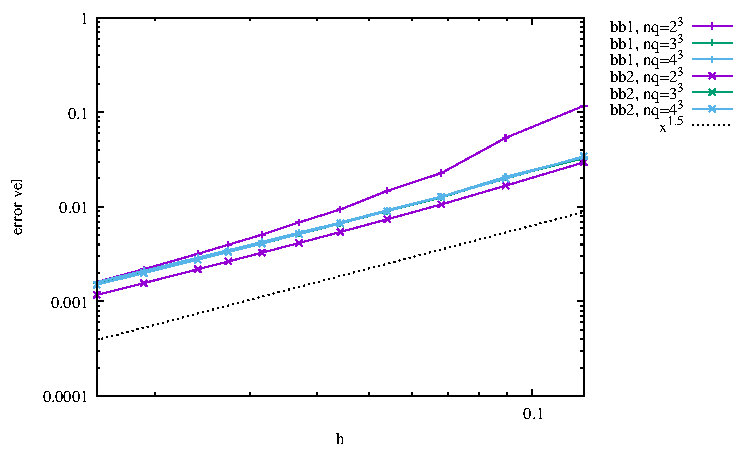
\includegraphics[width=8cm]{python_codes/fieldstone_75/results/burst/errors_v.pdf}
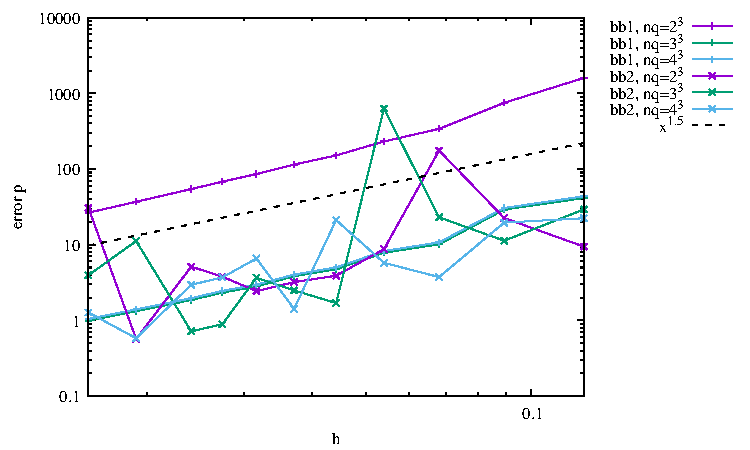
\includegraphics[width=8cm]{python_codes/fieldstone_75/results/burst/errors_p.pdf}\\
{\captionfont Velocity and pressure error convergence for both bubbles and with varying number of 
quadrature points nq.}
\end{center}


\begin{center}
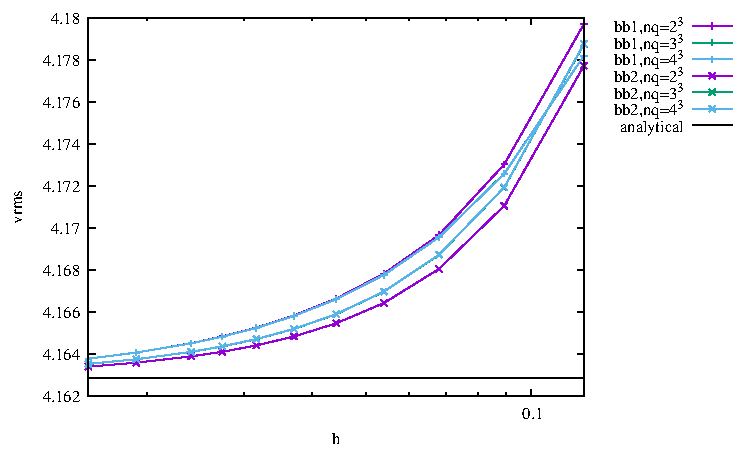
\includegraphics[width=8cm]{python_codes/fieldstone_75/results/burst/vrms.pdf}\\
{\captionfont Root mean square velocity for both bubbles and with varying number of   
quadrature points nq.}
\end{center}


\begin{center}
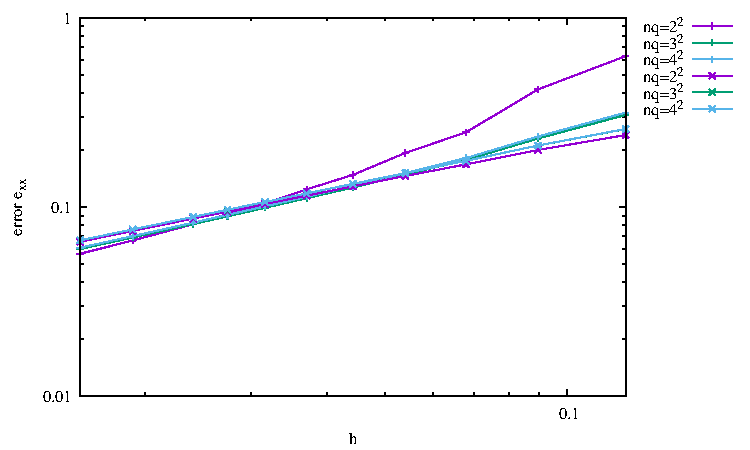
\includegraphics[width=5cm]{python_codes/fieldstone_75/results/burst/errors_exx}
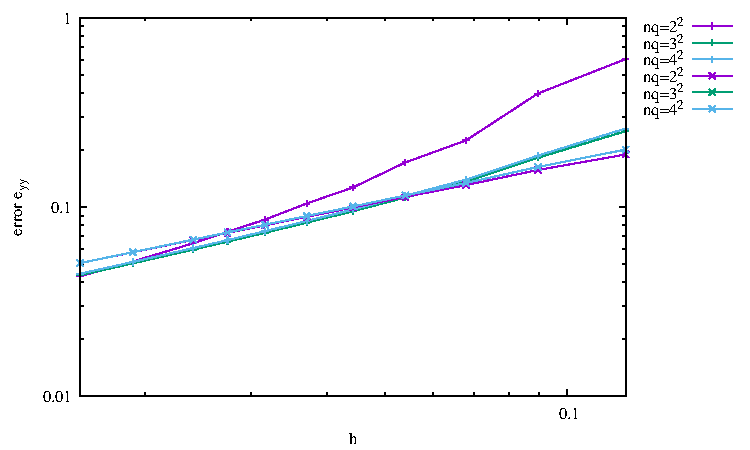
\includegraphics[width=5cm]{python_codes/fieldstone_75/results/burst/errors_eyy}
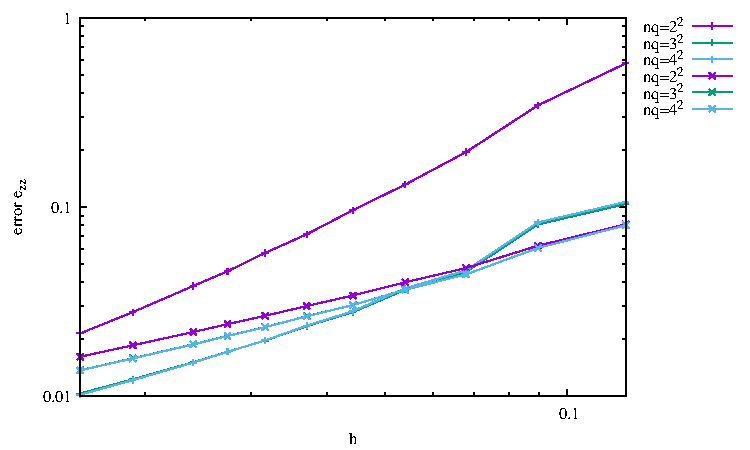
\includegraphics[width=5cm]{python_codes/fieldstone_75/results/burst/errors_ezz}\\
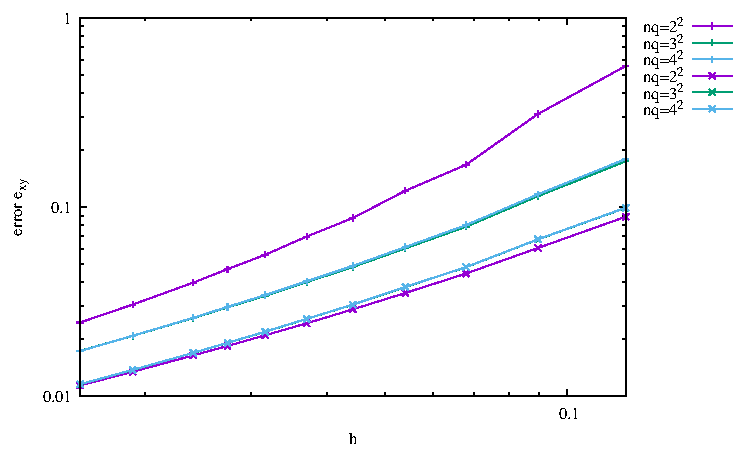
\includegraphics[width=5cm]{python_codes/fieldstone_75/results/burst/errors_exy}
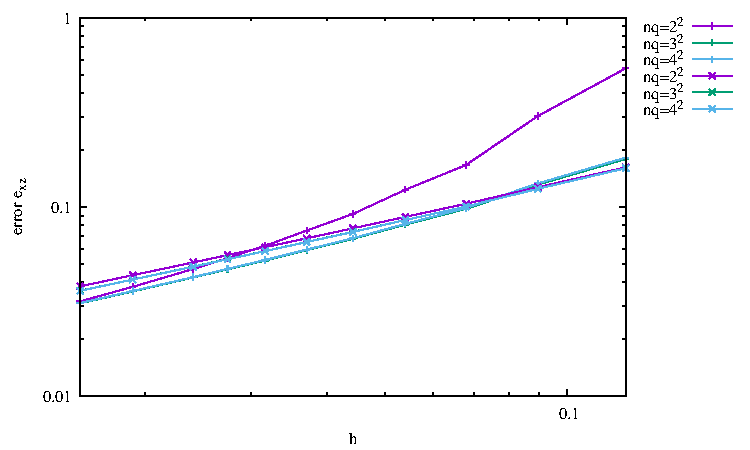
\includegraphics[width=5cm]{python_codes/fieldstone_75/results/burst/errors_exz}
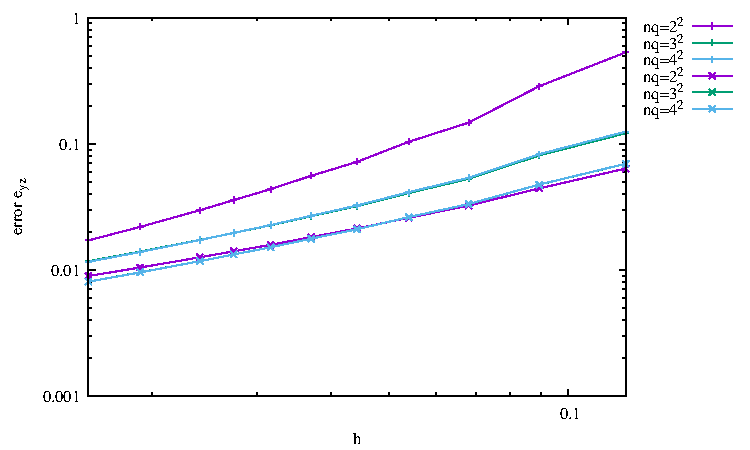
\includegraphics[width=5cm]{python_codes/fieldstone_75/results/burst/errors_eyz}\\
{\captionfont Error convergence for the 6 components of the strain rate tensor.}
\end{center}


\begin{center}
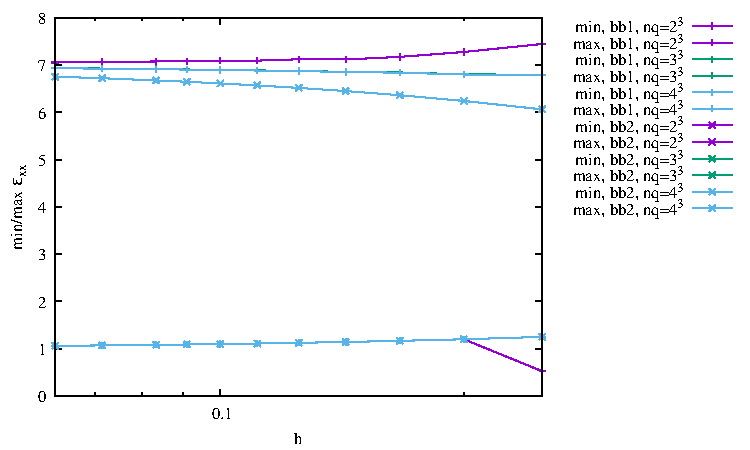
\includegraphics[width=5cm]{python_codes/fieldstone_75/results/burst/exx_stats.pdf}
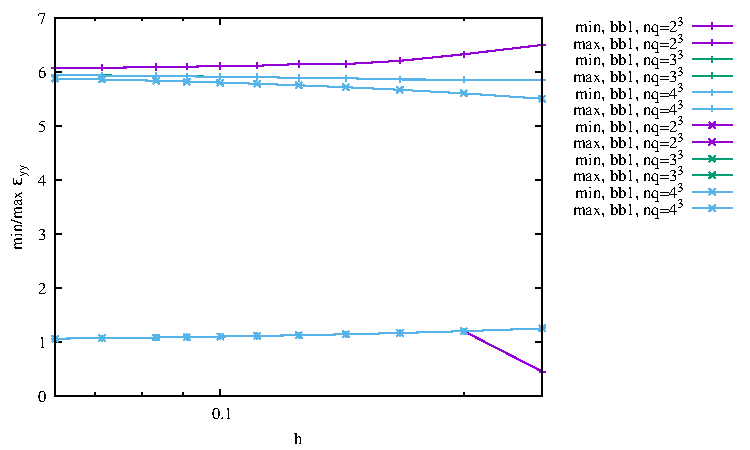
\includegraphics[width=5cm]{python_codes/fieldstone_75/results/burst/eyy_stats.pdf}
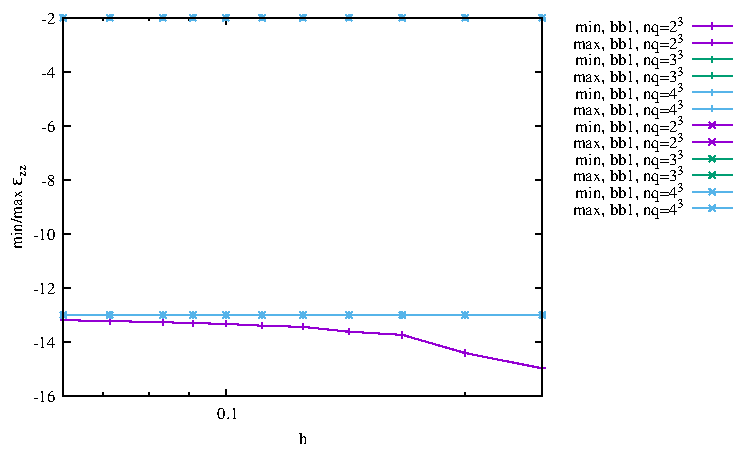
\includegraphics[width=5cm]{python_codes/fieldstone_75/results/burst/ezz_stats.pdf}\\
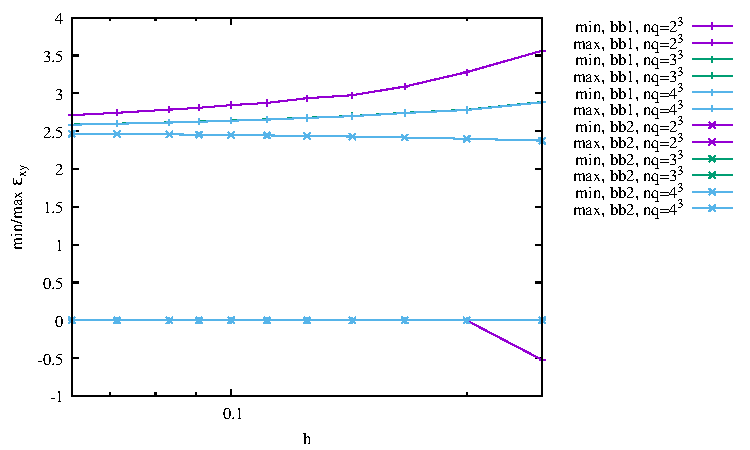
\includegraphics[width=5cm]{python_codes/fieldstone_75/results/burst/exy_stats.pdf}
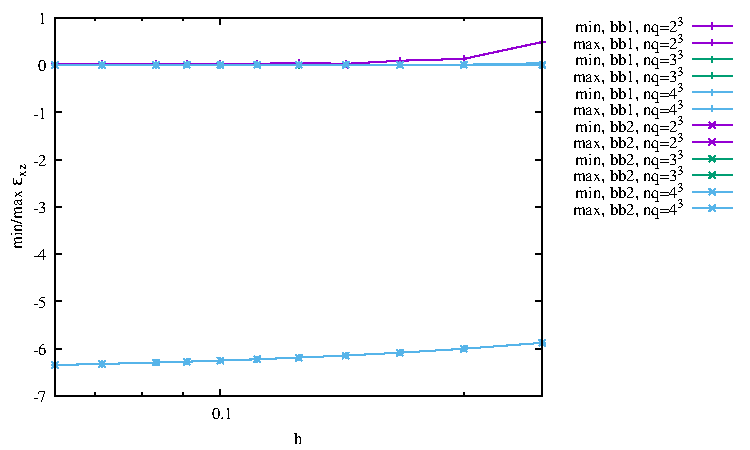
\includegraphics[width=5cm]{python_codes/fieldstone_75/results/burst/exz_stats.pdf}
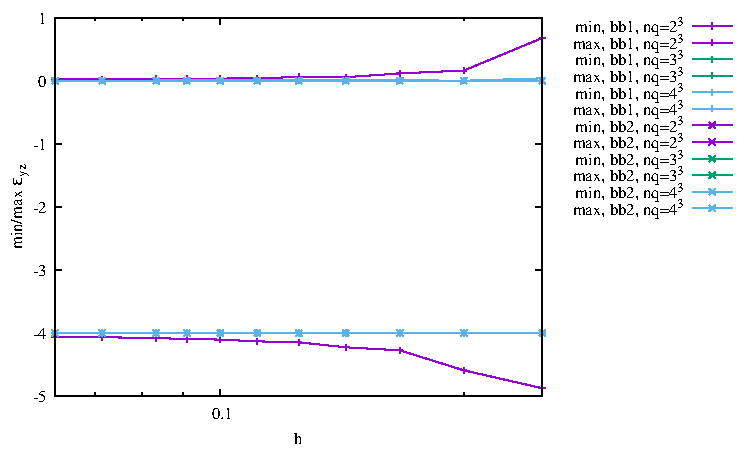
\includegraphics[width=5cm]{python_codes/fieldstone_75/results/burst/eyz_stats.pdf}\\
{\captionfont min/max statistics of the 6 components of the strain rate tensor
as a function of the mesh size $h$.}
\end{center}


\begin{center}
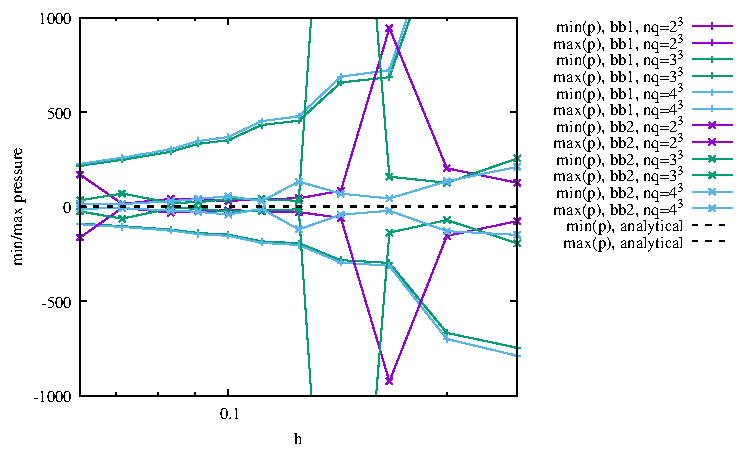
\includegraphics[width=11cm]{python_codes/fieldstone_75/results/burst/p_stats.pdf}\\
{\captionfont min/max statistics of the pressure as a function of the mesh size $h$. Note that 
the black dashed lines represent the analytical solution!}
\end{center}

\begin{center}
\includegraphics[width=5cm]{python_codes/fieldstone_75/results/burst/vel.png}
\includegraphics[width=5cm]{python_codes/fieldstone_75/results/burst/p_b1}
\includegraphics[width=5cm]{python_codes/fieldstone_75/results/burst/p_b2}\\
{\captionfont From left to right: velocity field; pressure field obtained with bubble 1;
pressure field obtained with bubble 2. Resolution is 12x12x12 elements.}
\end{center}

We see that in this case the bubble \#2 is way worse than bubble \#1. Both 
yield very bad pressure fields, although the pressure min/max value seem to converge 
towards the analytical values for bubble \#1. 
Note that the current code is limited to fairly low resolutions, i.e. about $24^3$ elements so that
I would need to implement a better Stokes solver (e.g. CG on Schur complement) instead 
of building the Stokes system and passing it to the solver as a whole as I do now. %Take it from stone 16. 

It appears that $3^3$ quadrature points always yield better results than $2^3$ points
so I set $nq=3^3$ in what follows.

\newpage
I have done a fair bit of exploration when it comes to bubbles.
In the end, and given our experience with the 2D ones, we expect them  
to be the natural extension of the 2D bubbles:
\[
b^0(r,s,t) = (1-r^2)(1-s^2)(1-t^2)
\]
\[
b^1(r,s,t) = (1-r^2)(1-s^2)(1-t^2)(1-r)(1-s)(1-t) 
\]
\[
b^2(r,s,t) = (1-r^2)(1-s^2)(1-t^2) (1+\beta(r+s+t))
\]
As I have done in \stone~\ref{f72}, I have created in {\tt study}
a simple code that creates a $2\times 2 \times 2$ mesh (a macro-element)
and looks at the null space and rank of the $\G$ matrix 
for these bubble functions.

The issue is that the mesh counts 3*3*3+8 nodes, i.e. NfemV=105 and 
NfemP=27 so that printing the $\G$ matrix is cumbersome. 
There are 26 nodes on the sides/edges so that 26*3=78 lines
of the $\G$ matrix will be entirely zero. In the end 
the $\G^\star$ matrix is of size $27\times 27$... 

%----------------------
\subsection*{bubble 0}

In this case the nullspace is given by
\begin{tiny}
\begin{verbatim}
[[-6.55615919e-02  1.44031044e-01  0.00000000e+00  0.00000000e+00  2.97645930e-01]
 [-6.76523164e-03 -2.60178381e-02  1.24864351e-01 -4.15781369e-01 -1.43523567e-02]
 [-6.55615919e-02  1.44031044e-01 -3.94785116e-16 -8.39823003e-16  2.97645930e-01]
 [-1.91177759e-01  2.51551355e-01 -1.98170968e-01 -1.20271118e-01 -1.89288260e-01]
 [-2.62530447e-01  1.06706899e-02  3.71268341e-01  2.24840853e-01 -1.20858682e-02]
 [-1.91177759e-01  2.51551355e-01 -1.98170968e-01 -1.20271118e-01 -1.89288260e-01]
 [-6.55615919e-02  1.44031044e-01 -2.02474756e-17  4.16767315e-16  2.97645930e-01]
 [-6.76523164e-03 -2.60178381e-02  1.24864351e-01 -4.15781369e-01 -1.43523567e-02]
 [-6.55615919e-02  1.44031044e-01 -8.93653641e-17 -3.63641409e-16  2.97645930e-01]
 [ 2.44846258e-02  2.60307508e-01  3.14515329e-01  2.81444969e-02 -1.46022049e-01]
 [-4.78192832e-01  1.91453680e-03 -1.41417956e-01  7.64252380e-02 -5.53520784e-02]
 [ 2.44846258e-02  2.60307508e-01  3.14515329e-01  2.81444969e-02 -1.46022049e-01]
 [-2.93780305e-01 -2.75654656e-01  1.81617363e-01 -2.19085013e-01  1.19583825e-01]
 [ 2.21453481e-01  3.93667862e-01 -5.67530121e-02 -1.96696356e-01  1.63709749e-01]
 [-2.93780305e-01 -2.75654656e-01  1.81617363e-01 -2.19085013e-01  1.19583825e-01]
 [ 2.44846258e-02  2.60307508e-01  3.14515329e-01  2.81444969e-02 -1.46022049e-01]
 [-4.78192832e-01  1.91453680e-03 -1.41417956e-01  7.64252380e-02 -5.53520784e-02]
 [ 2.44846258e-02  2.60307508e-01  3.14515329e-01  2.81444969e-02 -1.46022049e-01]
 [-6.55615919e-02  1.44031044e-01 -4.55825698e-16  2.59774841e-16  2.97645930e-01]
 [-6.76523164e-03 -2.60178381e-02  1.24864351e-01 -4.15781369e-01 -1.43523567e-02]
 [-6.55615919e-02  1.44031044e-01 -8.03014339e-16 -8.03014339e-16  2.97645930e-01]
 [-1.91177759e-01  2.51551355e-01 -1.98170968e-01 -1.20271118e-01 -1.89288260e-01]
 [-2.62530447e-01  1.06706899e-02  3.71268341e-01  2.24840853e-01 -1.20858682e-02]
 [-1.91177759e-01  2.51551355e-01 -1.98170968e-01 -1.20271118e-01 -1.89288260e-01]
 [-6.55615919e-02  1.44031044e-01 -6.81597248e-16  5.15429713e-16  2.97645930e-01]
 [-6.76523164e-03 -2.60178381e-02  1.24864351e-01 -4.15781369e-01 -1.43523567e-02]
 [-6.55615919e-02  1.44031044e-01 -7.82793969e-16 -3.43692089e-16  2.97645930e-01]]
\end{verbatim}
\end{tiny}

and the rank is 5.

%----------------------
\subsection*{bubble 1}

In this case the nullspace is given by
\begin{tiny}
\begin{verbatim}
[[ 0.         -0.23884962  0.          0.          0.08080294]
 [ 0.16934348  0.02392195 -0.03938398  0.22747521  0.14630426]
 [-0.21471563 -0.27040088 -0.02233311 -0.06461868  0.09425184]
 [-0.10673752  0.02892976  0.07100044  0.24642258  0.16110711]
 [-0.06591281 -0.23602745 -0.14788432 -0.17954949  0.18312833]
 [ 0.06791595  0.01165658  0.24348047  0.38573023  0.08079715]
 [ 0.13038563 -0.27666064 -0.16031363 -0.08830289  0.07574828]
 [ 0.17144633  0.00977865  0.20208631  0.37862496  0.07524609]
 [-0.18274347 -0.19525262 -0.43607008 -0.21124923  0.17994838]
 [-0.03432163  0.06536259 -0.13910722  0.08303938  0.26880082]
 [-0.17453665 -0.2906767   0.16727717  0.06552531  0.02158776]
 [ 0.23085171  0.09363046 -0.22926176  0.01811802  0.32310801]
 [ 0.23958486 -0.29818842  0.00170054  0.03710426 -0.00061651]
 [ 0.00764748  0.04207031 -0.04093494  0.19051424  0.18979327]
 [ 0.0629548  -0.24369011 -0.0715382   0.07091686  0.00812761]
 [-0.28680018  0.1030201  -0.02229098  0.05364434  0.35086335]
 [-0.09234076 -0.24087321 -0.00944696  0.08157475  0.01645422]
 [ 0.05486823 -0.06197475  0.11312173 -0.12609726  0.3621444 ]
 [ 0.03986577 -0.32220169  0.10232094  0.11592612 -0.05886886]
 [ 0.30722613  0.07809022 -0.19186555  0.07228145  0.2771718 ]
 [-0.38641316 -0.29771997  0.15485771  0.24826604 -0.12294019]
 [-0.31395614  0.08935779  0.0564994   0.11491304  0.31047821]
 [-0.05160682 -0.22037974 -0.12763252 -0.0103283   0.07703193]
 [-0.00623268 -0.09271495  0.29040007  0.01175732  0.27127783]
 [ 0.39006467 -0.31180443 -0.15559848  0.19497656 -0.1645732 ]
 [ 0.22671067 -0.09694029  0.19726322 -0.00422952  0.25878793]
 [-0.18660551  0.08617576 -0.54478139  0.54324418 -0.14236849]]
\end{verbatim}
\end{tiny}

and rank is 22

%----------------------
\subsection*{bubble 2}

$\beta=1/4$

In this case the nullspace is given by
\begin{tiny}
\begin{verbatim}
[[ 0.          0.26976967  0.        ]
 [ 0.27392841 -0.01117426 -0.09223388]
 [-0.00458301  0.25379735 -0.11621606]
 [ 0.27392841 -0.01117426 -0.09223388]
 [ 0.0093026   0.30219028  0.23589544]
 [ 0.27790582  0.00268746  0.00862534]
 [-0.00458301  0.25379735 -0.11621606]
 [ 0.27790582  0.00268746  0.00862534]
 [-0.01089738  0.23179104 -0.27633605]
 [ 0.27392841 -0.01117426 -0.09223388]
 [ 0.0093026   0.30219028  0.23589544]
 [ 0.27790582  0.00268746  0.00862534]
 [ 0.0093026   0.30219028  0.23589544]
 [ 0.26255856 -0.05079946 -0.38055052]
 [ 0.00606537  0.29090817  0.15380569]
 [ 0.27790582  0.00268746  0.00862534]
 [ 0.00606537  0.29090817  0.15380569]
 [ 0.28365743  0.0227325   0.1544749 ]
 [-0.00458301  0.25379735 -0.11621606]
 [ 0.27790582  0.00268746  0.00862534]
 [-0.01089738  0.23179104 -0.27633605]
 [ 0.27790582  0.00268746  0.00862534]
 [ 0.00606537  0.29090817  0.15380569]
 [ 0.28365743  0.0227325   0.1544749 ]
 [-0.01089738  0.23179104 -0.27633605]
 [ 0.28365743  0.0227325   0.1544749 ]
 [-0.01972214  0.20103577 -0.50011426]]
\end{verbatim}
\end{tiny}

and rank is 24

This is the 'best'. changing beta value does not change anything. 

%------------------------------------------
\subsection*{further systematic testing}
From the short study above we can conclude that the 
bubbles obtained by extending the 2D ones are 
not sufficient to stabilise the element in 3D.

We then postulate the bubble functions to be of the form
\[
b(r,s,t) = (1-r^2)(1-s^2)(1-t^2) {\cal P}(r,s,t)
\]
where ${\cal P}(r,s,t)$ is a low order polynomial, say
\[
{\cal P}(r,s,t) =  
1 + a_1r + b_1s + c_1t +
a_2 r^2  + b_2 s^2 + c_2 t^2 + 
d_2 rs   + e_2st + f_2rt +
a_3 r^3  + b_3 s^3 + c_3 t^3 + d_3 r^2s + e_3 r^2 t + f_3 r s^2 + g_3 s^2 t +
h_3 rt^2 + i_3 st^2 + j_3 rst
\] 
The question is then: is there such a polynomial that 
yields a stable element pair? 

I have therefore designed a bash script {\tt script\_bubblesearch}
that performs a large number of rank/nullspace calculations 
for many combinations of the polynomial coefficients.
There are 19 parameters. Even if I only try 2 values for each, I'll need to run
the code $2^{19}$ times... 

Let us start with the simple case $a_3=b_3=...=j_3=0$. Then the search space is much smaller.
We choose $a_1,b_1,c_2 \in \{0,0.25,1\}$, $a_2,..f_2\in \{ -1,0,1\}$ and $a_3=...j_3=0$.
We find that the size of the nullspace is always 3, 4 or 5 but not smaller.

Thought: is 2D, the macro element has 10 Vdofs left and 9 Pdfofs, the matrix is not square. in 3D, the macro element has 27 Vdofs left and 27 Pdofs, i.e. matrix is square. 

\newpage
%...........................................................................
\section*{The generic mms3D} In order to verify that 
the above results are robust (or that I have not made a mistake)
I have tried another manufactured solution, as defined in Section~\ref{MMM-ss:mms3Dgen}. 
Python file on github is {\pythonfile stone\_mms3D.py}

\begin{eqnarray}
u(x,y,z) &=& x(1-x)(1-2y)(1-2z)\\
v(x,y,z) &=& (1-2x) y(1-y) (1-2z) \\
w(x,y,z) &=& -2(1-2x)(1-2y)z(1-z) \\
p(x,y,z) &=& (2x-1)(2y-1)(2z-1)
\end{eqnarray}

\begin{center}
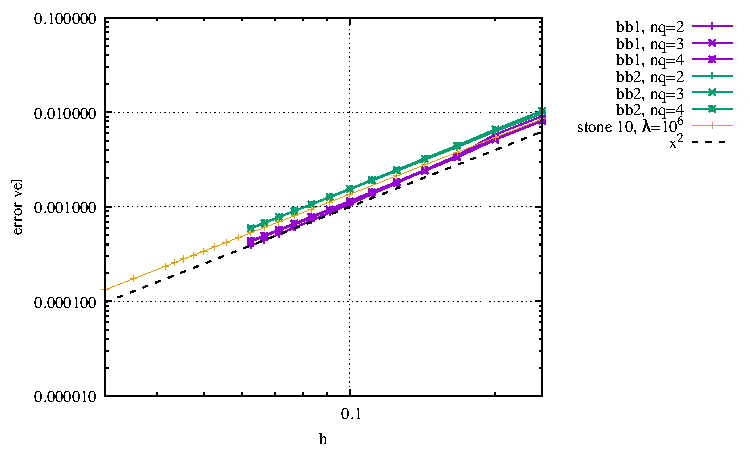
\includegraphics[width=7cm]{python_codes/fieldstone_75/results/mms3D/errorsV.pdf}
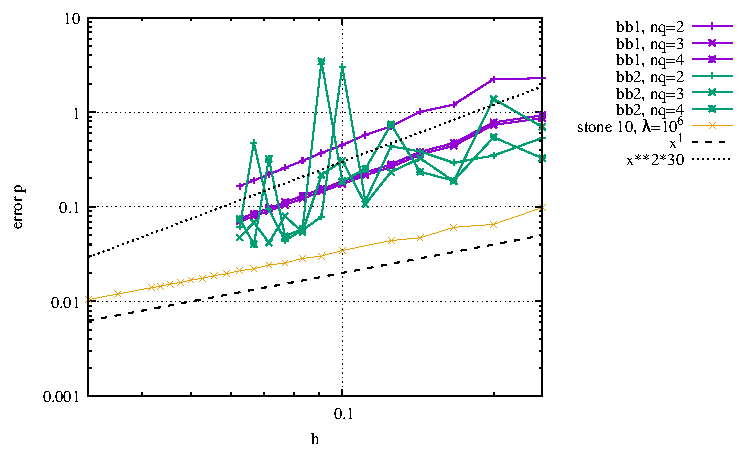
\includegraphics[width=7cm]{python_codes/fieldstone_75/results/mms3D/errorsP.pdf}\\
{\captionfont $\uparrow$ Velocity and pressure error convergence for both bubbles}
\end{center}

\begin{center}
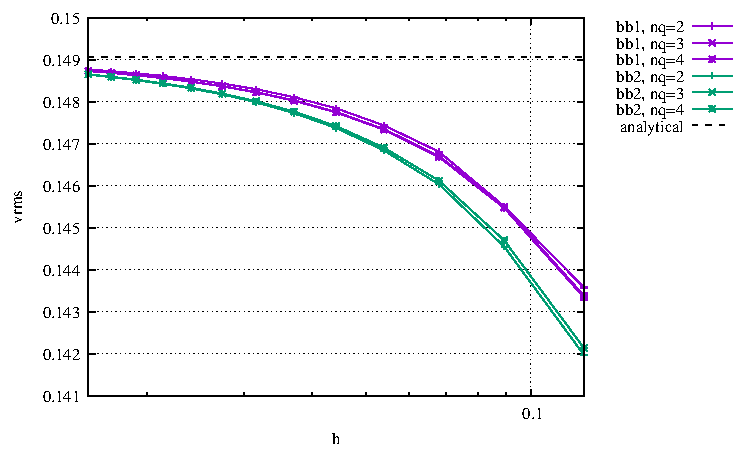
\includegraphics[width=8cm]{python_codes/fieldstone_75/results/mms3D/vrms.pdf}\\
{\captionfont $\uparrow$ Root mean square velocity for both bubbles}
\end{center}

%\begin{center}
%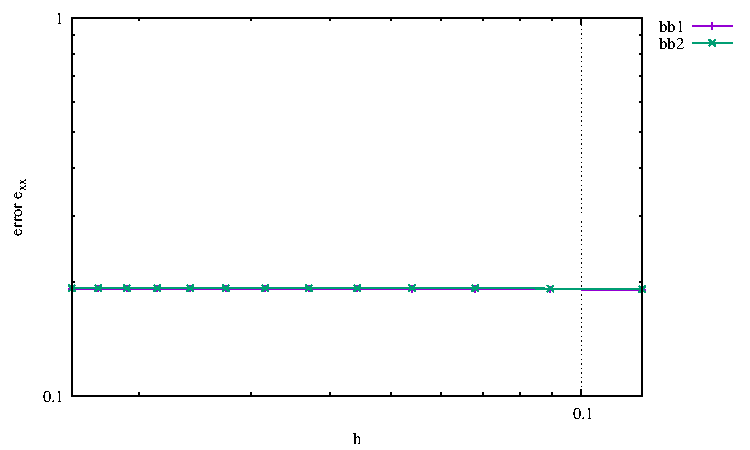
\includegraphics[width=5cm]{python_codes/fieldstone_75/results/mms3D/errors_exx}
%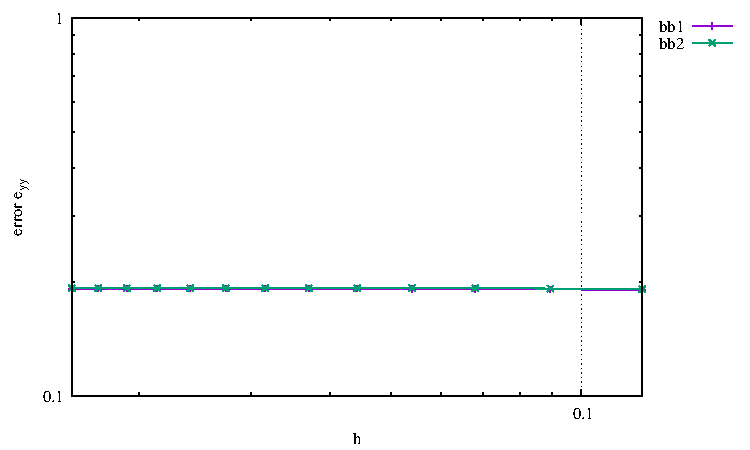
\includegraphics[width=5cm]{python_codes/fieldstone_75/results/mms3D/errors_eyy}
%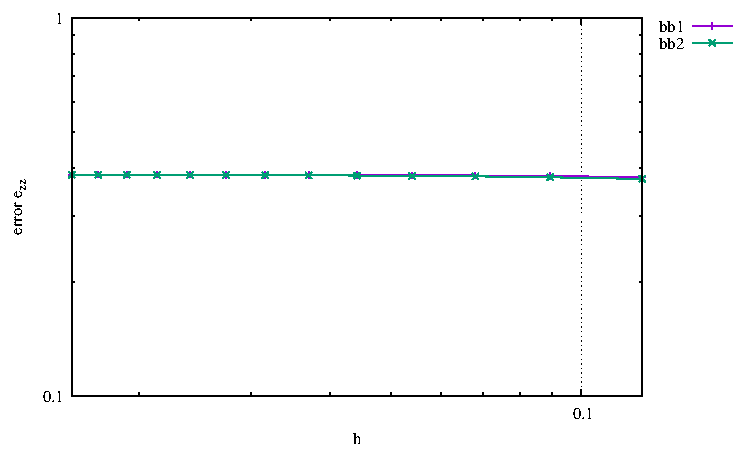
\includegraphics[width=5cm]{python_codes/fieldstone_75/results/mms3D/errors_ezz}\\
%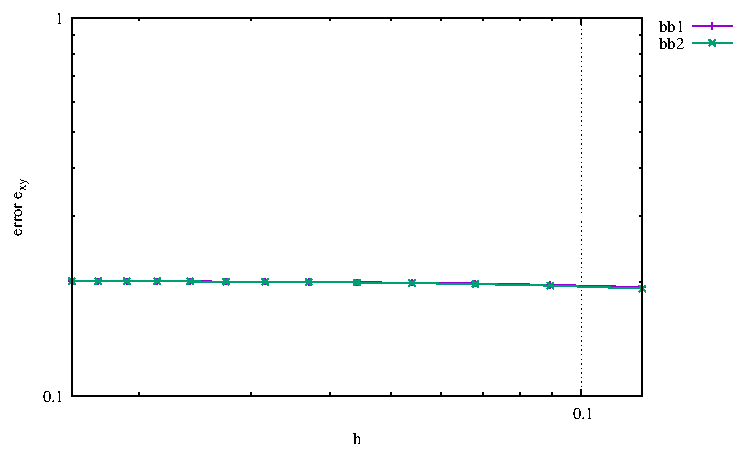
\includegraphics[width=5cm]{python_codes/fieldstone_75/results/mms3D/errors_exy}
%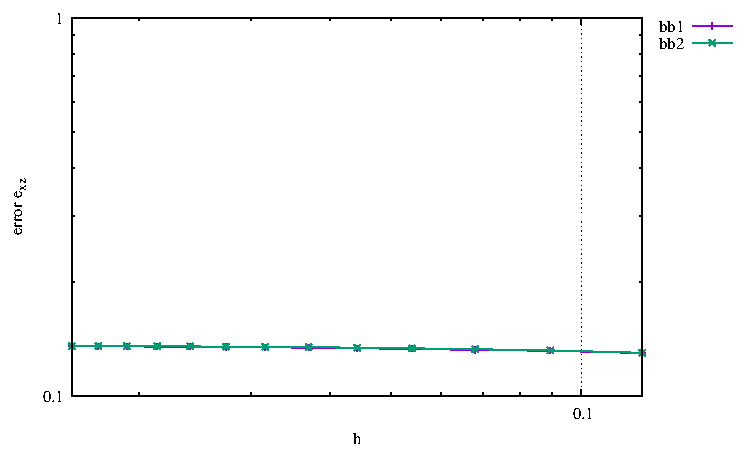
\includegraphics[width=5cm]{python_codes/fieldstone_75/results/mms3D/errors_exz}
%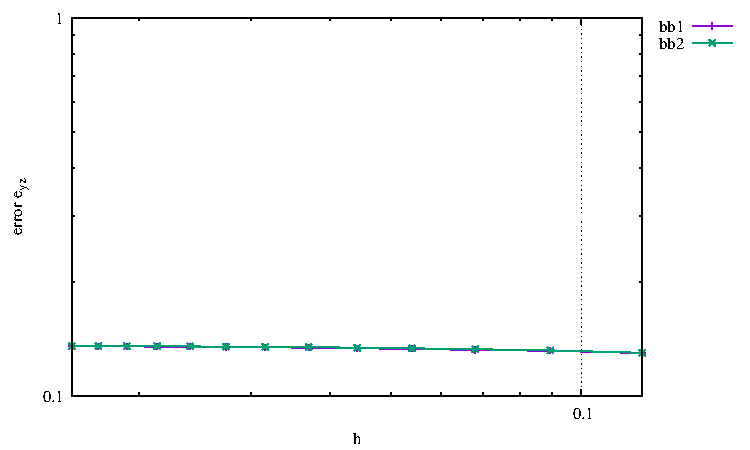
\includegraphics[width=5cm]{python_codes/fieldstone_75/results/mms3D/errors_eyz}\\
%{\captionfont $\uparrow$ Error convergence for the 6 components of the strain rate tensor.}
%\end{center}

%\begin{center}
%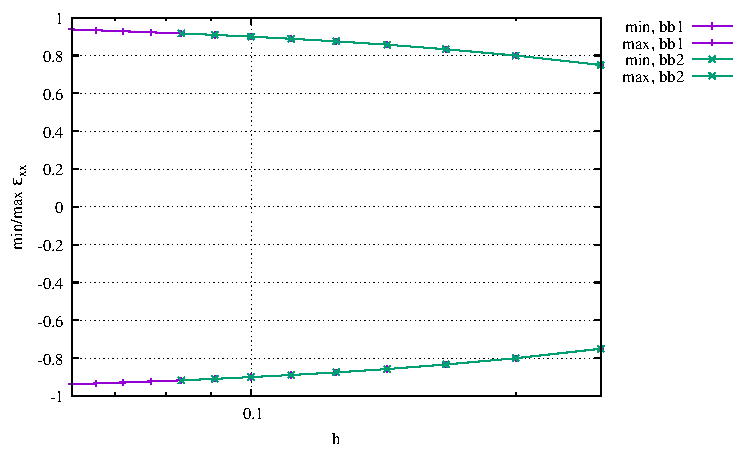
\includegraphics[width=5cm]{python_codes/fieldstone_75/results/mms3D/exx_stats.pdf}
%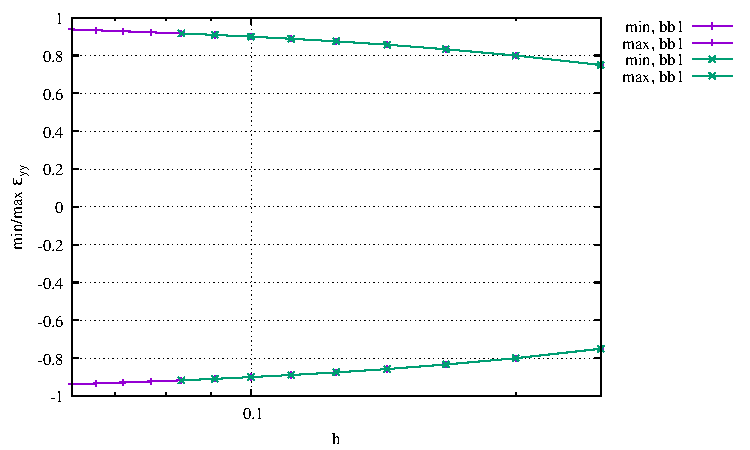
\includegraphics[width=5cm]{python_codes/fieldstone_75/results/mms3D/eyy_stats.pdf}
%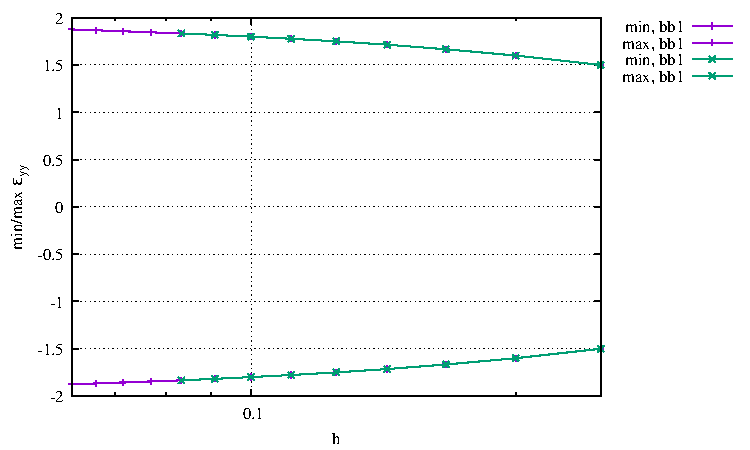
\includegraphics[width=5cm]{python_codes/fieldstone_75/results/mms3D/ezz_stats.pdf}\\
%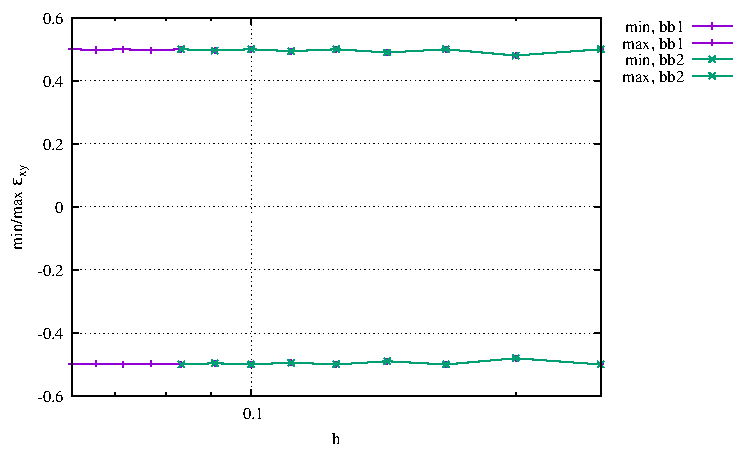
\includegraphics[width=5cm]{python_codes/fieldstone_75/results/mms3D/exy_stats.pdf}
%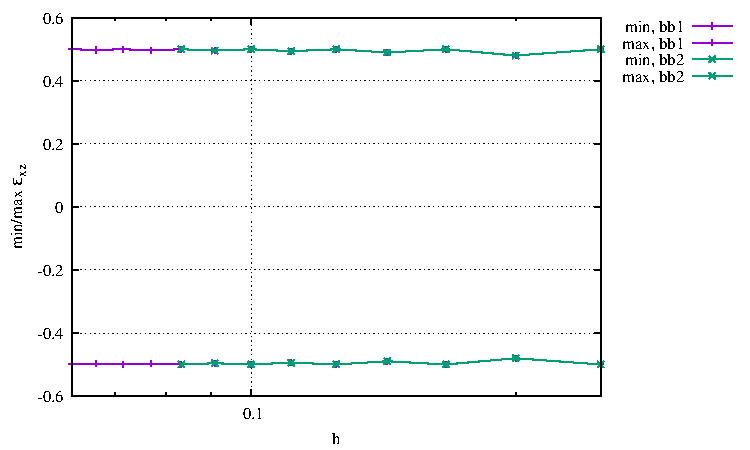
\includegraphics[width=5cm]{python_codes/fieldstone_75/results/mms3D/exz_stats.pdf}
%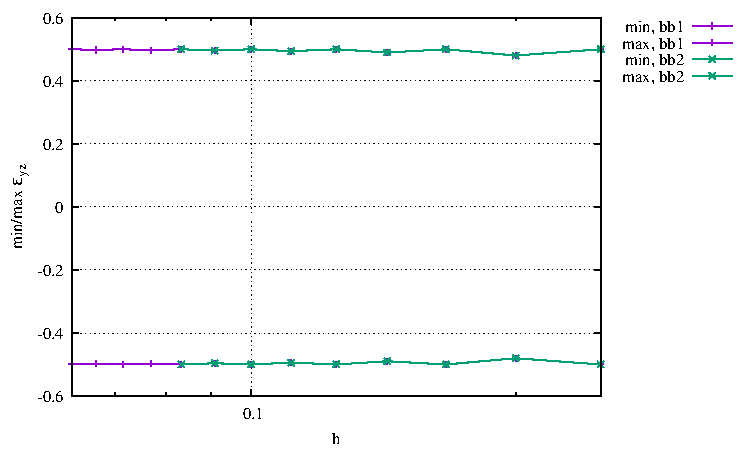
\includegraphics[width=5cm]{python_codes/fieldstone_75/results/mms3D/eyz_stats.pdf}\\
%{\captionfont $\uparrow$ min/max statistics of the 6 components of the strain rate tensor
%as a function of the mesh size $h$.}
%\end{center}


\begin{center}
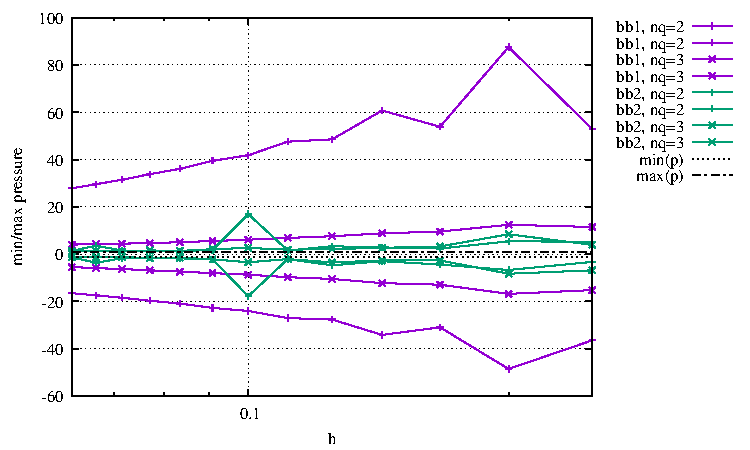
\includegraphics[width=11cm]{python_codes/fieldstone_75/results/mms3D/p_stats.pdf}\\
{\captionfont $\uparrow$ min/max statistics of the pressure as a function of the mesh size $h$.}
\end{center}


%\begin{center}
%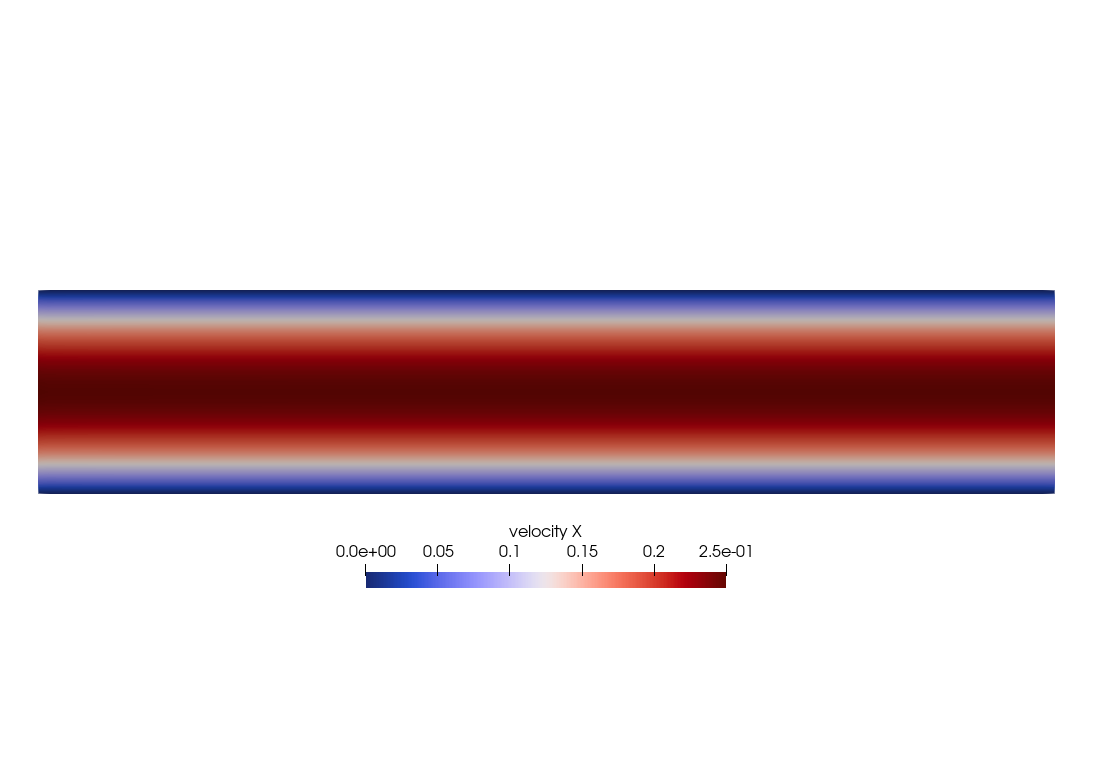
\includegraphics[width=5cm]{python_codes/fieldstone_75/results/mms3D/u}
%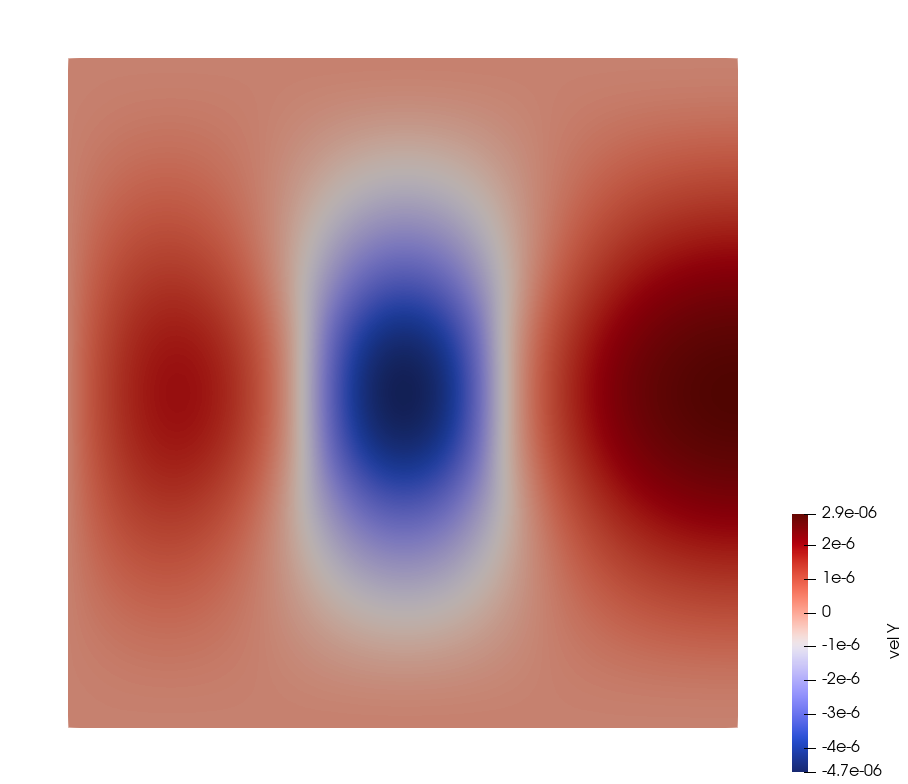
\includegraphics[width=5cm]{python_codes/fieldstone_75/results/mms3D/v}
%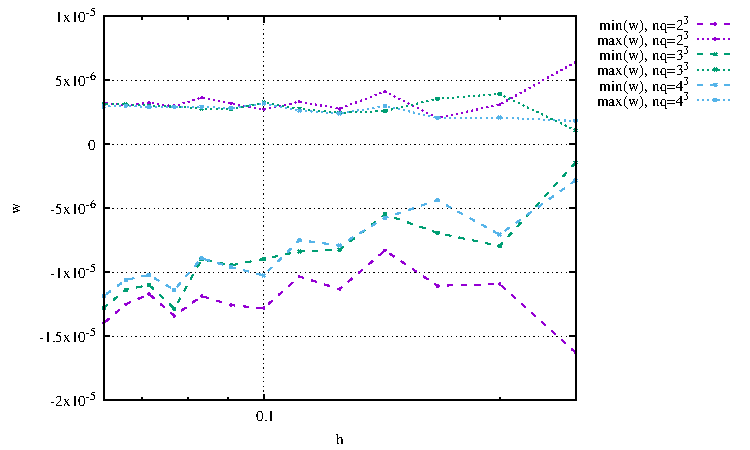
\includegraphics[width=5cm]{python_codes/fieldstone_75/results/mms3D/w}\\
%\includegraphics[width=5cm]{python_codes/fieldstone_75/results/mms3D/vel}
%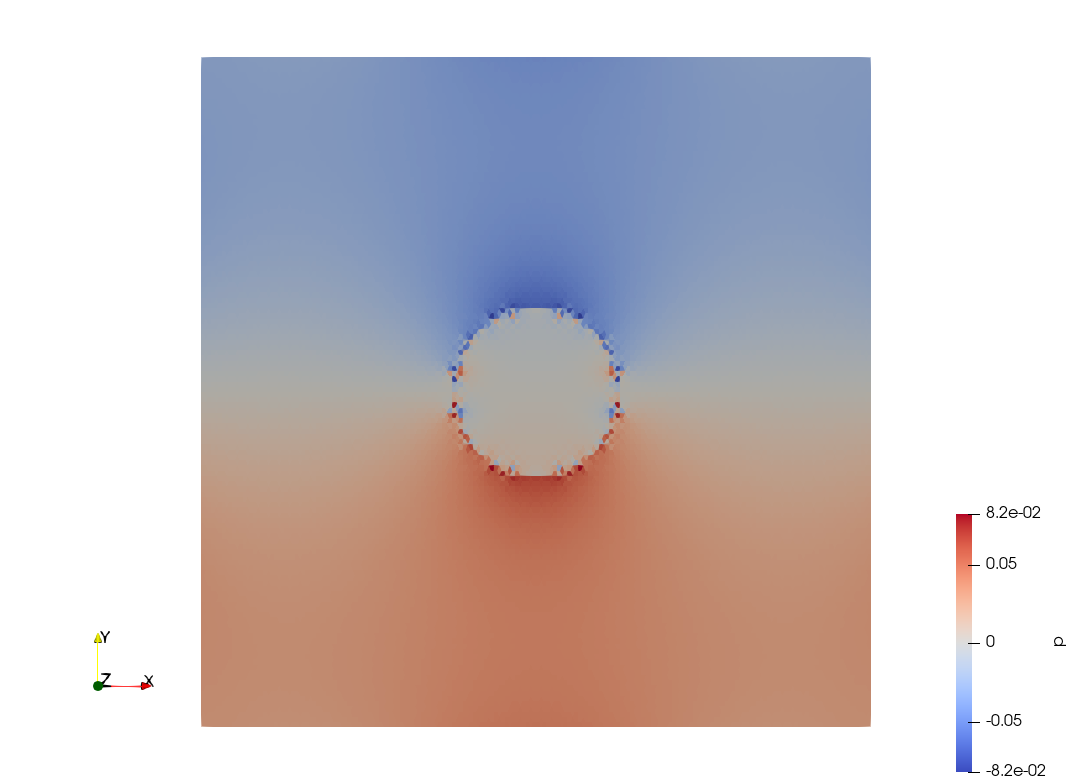
\includegraphics[width=5cm]{python_codes/fieldstone_75/results/mms3D/p}\\
%{\captionfont $\uparrow$ Velocity and pressure fields (analytical fields)}
%\end{center}

%\begin{center}
%\includegraphics[width=7cm]{python_codes/fieldstone_75/results/mms3D/p_b1}
%\includegraphics[width=7cm]{python_codes/fieldstone_75/results/mms3D/p_b2}\\
%{\captionfont Pressure field. Left: bubble \#1, Right: bubble \#2.}
%\end{center}

Once again, the conclusion is clear: none of the two bubbles is capable of generating a 
smooth pressure field. Bubble 1 is objectively better than bubble 2.
It could be that my conclusions are limited by the lack of high resolution measurements
but the 2D experiments with the equivalent bubbles worked fine at low resolution...

The nail in the coffin comes from Remark 1 of \textcite{kahp20}:
"Contrary to the two-dimensional case studied
in \textcite{bai97} (1997) and \textcite{lami17} (2017) it is not sufficient to enrich the 
standard isoparametric finite element space for hexahedrons with only one
bubble function. In this case both the spaces $V_{0,M_i}$ and $P_{M_i}$
have a dimension of 27, however, matrix D has only rank 24."

The answer to how to continue further is in \stone~\ref{f82}.
